\chapter{Word embeddings}
In this chapter, we will discuss ways of representing text numerically, how we can create word embeddings and details around the word2vec technique from architectural choices to data preprocessing. Furthermore, we will explain word2vec as an artificial neural network and at last, cover evaluation of word2vec models.

\section{Numerical representation of text}
Machine learning methods take in vectors (arrays of numbers) as input. When we want to work with text, we have to come up with some procedure for converting text into a vector, (i.e. vectorizing the text).
In this section, we will create some unique representation for words in a text, discuss one-hot encoding of words and the motivation behind creating word embeddings.

\subsection{Unique representation for each word}
\label{unique-representation-for-each-word}
A first strategy for vectorizing text could be to assign a unique number for each word in the text. We use the same order as the words appear in the text to assign a unique number. Furthermore, we define the number of unique words in the text to be the vocabulary size, denoted by $|V|$. We replace each word in the text with its respective number. Let us consider the following sentence
\begin{align}
    \text{the cat sat on the mat} \label{txt:num-rep-ex-sent-words}
\end{align}

We convert the words into numbers based on the order they appear in the text, e.g., the $\mapsto$ 0, cat $\mapsto$ 1, sat $\mapsto$ 2, etc.
\begin{align}
    \text{0 1 2 3 0 4} \label{txt:num-rep-ex-sent}
\end{align}
We now have a numerical representation of the original sentence in $\cref{txt:num-rep-ex-sent-words}$ and may use it for machine learning modeling.

There are some problems with this method, however.
\begin{itemize}
    \item The encoding of words into number is arbitrary (does not capture any relationship between words)
    \item Machine learning models might learn some natural ordering of the encodings, which can lead to bad results during inference. This is because the encoding of the words does not capture relationship between the words.
\end{itemize}

In the next subsection, we will look at another method of encoding words, using one-hot encodings. We will also apply it to the example sentence in \cref{txt:num-rep-ex-sent-words}.

\subsection{One-hot encoded words}
One-hot encoding is a method for converting categorical data into numeric data. Essentially, we create a unique, sparse vector consisting of all zeros, except for the value at the index of the element of interest, which we set to one. For instance, if we have the words "north", "east", "south", "west", then their one-hot encodings could be
\begin{align}
    \text{north} \mapsto \begin{pmatrix}
    1\\
    0\\
    0\\
    0
    \end{pmatrix},
    \text{east} \mapsto \begin{pmatrix}
    0\\
    1\\
    0\\
    0
    \end{pmatrix},
    \text{south} \mapsto \begin{pmatrix}
    0\\
    0\\
    1\\
    0
    \end{pmatrix},
    \text{west} \mapsto \begin{pmatrix}
    0\\
    0\\
    0\\
    1
    \end{pmatrix}
\end{align}

\begin{definition}
Let $V = \left \{ w_1, w_2, ..., w_{|V|} \right \}$ denote the set of unique words in a text. Then, the one-hot encoding of a word, $e_{w_i}$, is defined as a $|V|$-dimensional vector of all zeros, except for the value at index $i$ which is one. \label{def:one-hot-encoding}
\end{definition}

If we convert the words from  \cref{txt:num-rep-ex-sent-words} using \cref{def:one-hot-encoding}, we get the following one-hot encoded vectors
\begin{align}
    \begin{pmatrix}
    1\\
    0\\
    0\\
    0\\
    0
    \end{pmatrix}
    \begin{pmatrix}
    0\\
    1\\
    0\\
    0\\
    0
    \end{pmatrix}
    \begin{pmatrix}
    0\\
    0\\
    1\\
    0\\
    0
    \end{pmatrix}
    \begin{pmatrix}
    0\\
    0\\
    0\\
    1\\
    0
    \end{pmatrix}
    \begin{pmatrix}
    1\\
    0\\
    0\\
    0\\
    0
    \end{pmatrix}
    \begin{pmatrix}
    0\\
    0\\
    0\\
    0\\
    1
    \end{pmatrix}
\end{align}

We now have discarded the ordinal relationship of the numerical representation.

There are some downsides with this approach as well, however.
\begin{itemize}
    \item As with the numerical representation in \cref{unique-representation-for-each-word}, one-hot encoded vectors does not capture relationship between words.
    \item One-hot encoded vectors are sparse (meaning, most values are zero). Imagine if we had 1000 words in the vocabulary, then one would create a vector consisting of 99.9\% zeros. In practice, the vocabulary size is in the terms of $10^5$ to $10^7$ \cite{mikolov2013b}, i.e., by using one-hot encoded vector representations we are extremely inefficient in terms of space. We note, however, that there exists efficient methods for dealing with sparse vectors.
    \item One-hot encoded vectors are very high-dimensional (same as the number of words in the vocabulary, $|V|$).
\end{itemize}

\subsection{Word embeddings}
In contrast to the one-hot encoded vectors of words, word embeddings are low-dimensional dense vector representations. Word embeddings are typically learned from the data (e.g. texts) directly, whereas one-hot encoded vectors are arbitrarily defined (its ordering may change). Due to the lower dimensionality of word embeddings, it packs more information about words into less space, thus being more efficient than one-hot encoded word vectors. Common choices for the dimensionality of word embeddings are ranging from 50 to 600 \cite{mikolov2013a}, depending on the amount of training data. We will take a look at a classic family of methods of creating such word embeddings, called word2vec.

\section{Creating word embeddings (word2vec)}
Word2vec was first introduced by Mikolov et al. in 2013 \cite{mikolov2013a}. It is a family of techniques for learning dense and efficient vector representations of words. In the same year, Mikolov et al. introduced another paper which included several extensions that improved both the quality of the word embeddings and the training speed \cite{mikolov2013b}. In this section, we will go over the details of the original word2vec paper and the introduced extensions in the follow-up paper.

\subsection{Architectures}
The authors of the word2vec paper introduced two new log-linear models for learning distributed representations of words that try to minimize computational complexity, namely the continuous bag-of-words model (CBOW) and the continuous Skip-gram model. Both models achieve high quality (see \cref{sec:eval-word2vec-model} for evaluation of word2vec models) word embeddings \cite{mikolov2013a} and share some core idea as to how one might create good vector representations of words. In this subsection, we will go through both models.

\subsubsection{Continuous bag-of-words model}
The continuous bag-of-words model (CBOW) tries to predict a target word given some context words around it. Essentially, we select a target word $w_t$, where $t$ is the index of the current target word in our training data, and a number $C$ denoting the number of words to the left and to the right of $w_t$. $C$ is also called the window size. By combining the embedded context word vectors, we predict the target word $w_t$. This model is illustrated in \cref{fig:cbow-model}.

\begin{figure}[ht]
    \centering
    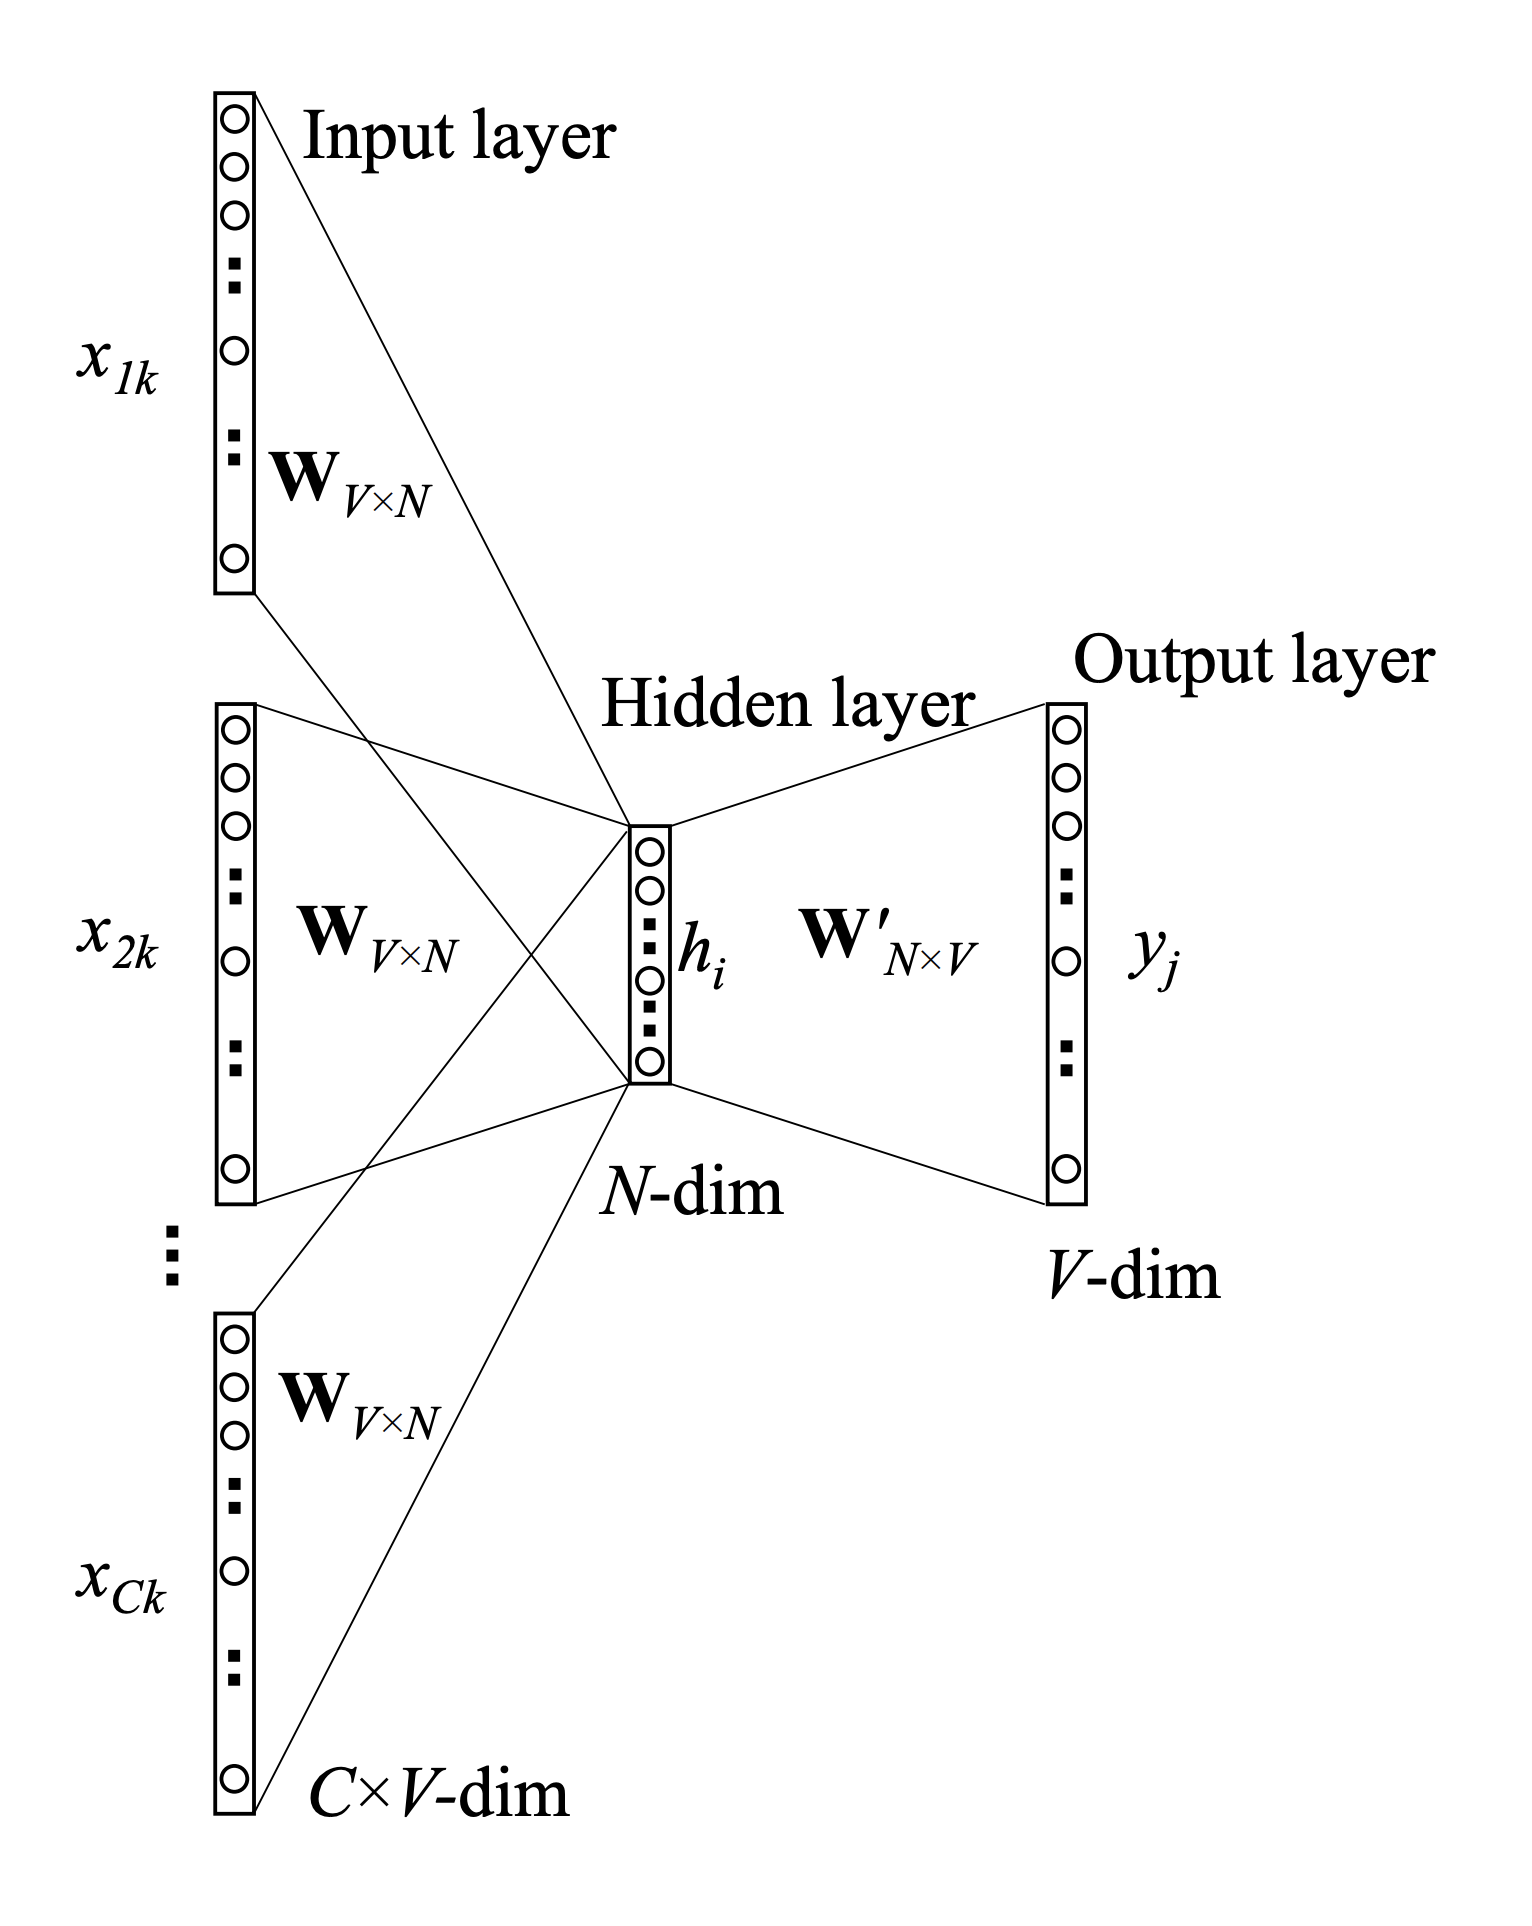
\includegraphics[width=8cm]{thesis/figures/cbow-rong-2016.png}
    \caption{CBOW architecture as illustrated by \cite{rong2016word2vec}}.
    \label{fig:cbow-model}
\end{figure}

More formally, we are considering a sequence of $T$ training words $w_1, w_2, \ldots, w_T$. The words $w_t$ belong to some vocabulary $V$ consisting of $|V|$ unique words, $1 \leq t \leq T$. The models task is to maximize the average log probability of the word $w_t$ being sampled given the context words $w_{t-C}, \ldots, w_{t-1}, w_{t+1}, \ldots, w_{t+C}$. The objective of the CBOW model then becomes
\begin{align}
    \frac{1}{T} \sumlim{t=1}{T} \log p(w_t | w_{t-C}, \ldots, w_{t-1}, w_{t+1}, \ldots, w_{t+C})
    \label{eqn:cbow-objective-function}
\end{align}

Through it is not clear from the original authors of word2vec \cite{mikolov2013a, mikolov2013b}, we typically use two weight matrices, $W$ and $W'$, when setting up the word2vec model \cite{rong2016word2vec}. The first weight matrix, $W$, is a $|V| \times D$ matrix, mapping the input word vectors (usually represented using one-hot encodings) to their internal embedding, where $|V|$ is the vocabulary size and $D$ is the number of dimensions in the embedding layer. The second weight matrix, $W'$, is a $D \times |V|$ matrix mapping from the embedding layer to the output prediction.

\subsubsection{Continuous Skip-gram model}
The continuous Skip-gram model is very similar to CBOW. In fact, the Skip-gram model tries to do the opposite; instead of predicting a target word given some context words, it tries to predict context words given some target word. Note that the ordering of the predicted context words does not matter. The Skip-gram model is illustrated in \cref{fig:skip-gram-model}.

\begin{figure}[ht]
    \centering
    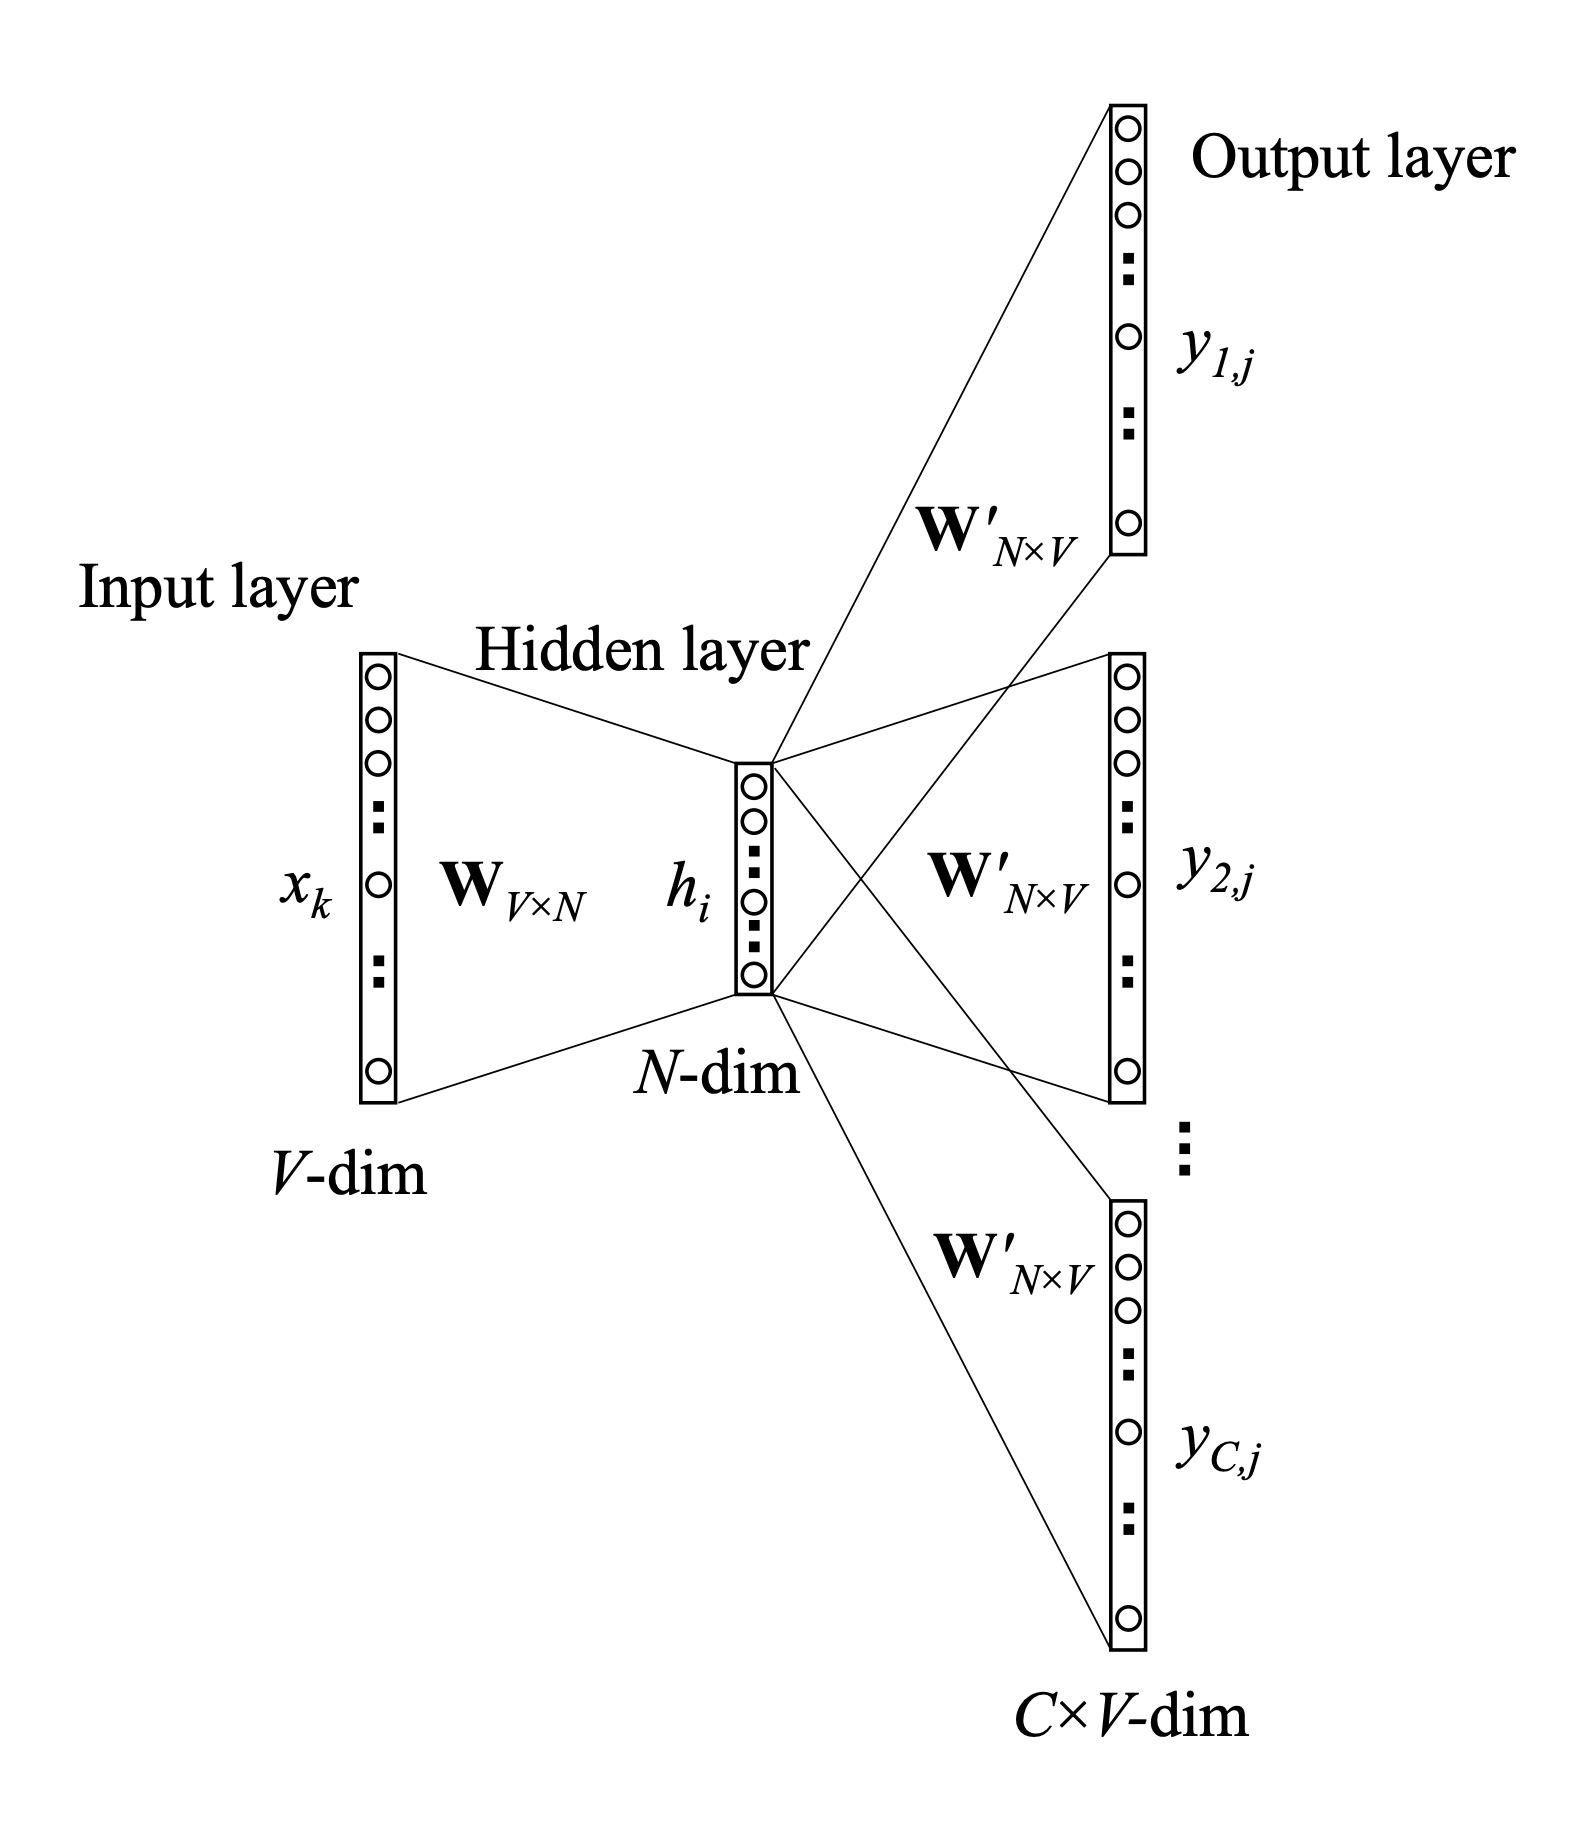
\includegraphics[width=8cm]{thesis/figures/skip-gram-rong-2016.png}
    \caption{The Skip-gram architecture as illustrated by  \cite{rong2016word2vec}. Note that the vectors from the output layers are unordered, i.e., we only want to predict that a given word belongs to its contextual words.}
    \label{fig:skip-gram-model}
\end{figure}

With the Skip-gram model, we also have some target word $w_t$ and context words around it. Let $C$ be the maximal distance from a target word to its contextual words. For each input to the model, we randomly sample a number $R$ in the range $[1, C]$ and denote this as the context size \cite{mikolov2013a}. In other words, for each target word $w_t$ we have $R$ context words around it, $w_{t-R}, \ldots, w_{t-1}, w_{t+1}, \ldots, w_{t+R}$. The objective of the Skip-gram model \cite{mikolov2013b} then becomes
\begin{align}
    \frac{1}{T} \sumlim{t=1}{T} \sumlim{-R \leq j \leq R, j \neq 0}{} \log p(w_{t+j} | w_t)
    \label{eqn:skip-gram-objective-function}
\end{align}
More generally, we define the objective of the Skip-gram model as such
\begin{align}
    \frac{1}{T} \sumlim{t=1}{T} \sumlim{w_O \in cw(w_I)}{} \log p(w_O | w_I)
    \label{eqn:skip-gram-objective-function-general}
\end{align}
where $w_I$ is the input word (e.g. target word), $w_O$ is the output word (e.g. context word) and $cw(w_I)$ is a function which returns the context words around input word $w_I$.

Similar to CBOW, the Skip-gram model uses the two matrices $W$ and $W'$ for mapping from input to embedding layer and embedding layer to output respectively.

Mikolov et al. reported that the Skip-gram model performed better than the CBOW model overall \cite{mikolov2013a}. For this reason and due to the scope of the masters thesis, we will stick to using the Skip-gram model throughout the thesis.

\subsection{Negative Sampling}
In the Skip-gram model, we typically define $p(w_O | w_I)$ using the softmax function \cite{mikolov2013b} \textbf{TODO: Reference softmax function?}
\begin{align}
    p(w_O | w_I)
    &= \frac{\exp{ \left( \trans{v'_{w_O}} v_{w_I} \right) }} {\exp{ \sumlim{k=1}{|V|} \left( \trans{v'_{w_k}} v_{w_I} \right) }}
    \label{eqn:skip-gram-p-function}
\end{align}
where $v_w$ and $v'_w$ are the "input" and "output" vector representations of the word $w$, and $|V|$ is the number of words in the vocabulary. There are some downsides with this formulation, however. In practice, it becomes hard to compute since the summation in the denominator of \cref{eqn:skip-gram-p-function} depends on the number of words in the vocabulary, which is often large ($10^5 - 10^7$ terms) \cite{mikolov2013b}.

To deal with the computational requirements of the original Skip-gram model, Mikolov et al. first showed how one might use hierarchical softmax \cite{mikolov2013b}. Hierarchical softmax is an efficient way of computing the softmax function; instead of evaluating $|V|$ words to compute the probability in \cref{eqn:skip-gram-p-function}, we only have to evaluate $\log \left( |V| \right)$ words \cite{mikolov2013b}.

As an alternative to hierarchical softmax, Mikolov et al. introduced negative sampling. Negative sampling builds on the concept of distinguishing target words $w_t$ from words randomly sampled from the vocabulary. In particular, we randomly sample words from the vocabulary using the unigram distribution raised to the power of $\alpha$ \cite{mikolov2013b}. The unigram distribution is a distribution for sampling a word at random from the vocabulary using the word occurrence counts, and the choice of raising it to the power of $\alpha = \frac{3}{4}$ was empirically found to be the best exponent. Furthermore, we will refer to this unigram distribution as the noise distribution $P_n(w)$ \cite{mikolov2013b}. Note that negative sampling method can also be applied to CBOW in a similar manner \cite{mikolov2013b}.

Before we can explain negative sampling, we define the positive- and negative target-context pairs.
\begin{definition}
Given a vocabulary $V$, a target word $w_t$ and the target words contextual words $w_{t-R}, \ldots, w_{t-1}, w_{t+1}, \ldots, w_{t+R}$ for some window size $R$, we define a \textbf{positive target-context pair} to be the pair of the target word $w_t$ and a contextual word $w_{t+j}$, $-R \leq j \leq R, j \neq 0$, i.e., the pair $\left( w_t, w_{t+j} \right)$. Furthermore, we define a \textbf{negative target-context pair} as the pair of the target word $w_t$ and a word $w_r$ randomly sampled from the noise distribution $P_n(w)$, i.e., the pair $\left( w_t, w_r \right)$.
\end{definition}

In negative sampling, we are only concerned with a subset of all the words in the vocabulary when computing the loss using the softmax function. For each word in the text we are training on, we create a positive target-context pair $\left( w_t, w_{t+j} \right)$, $-R \leq j \leq R, j \neq 0$. Furthermore, we generate $k$ negative target-context pairs for each word, where $k$ is in the range of $5-20$ for small training sets and $2-5$ for big training sets \cite{mikolov2013b}. We let $W_{np} = \left \{ w_i | i \in 1, \ldots, k \right \}$ be the set of $k$ negatively sampled words from the noise distribution $P_n(w)$. With these details in mind, the objective of negative sampling becomes \cite{mikolov2013b, rong2016word2vec}.
\begin{align}
    \log \sigma \left( \trans{v'_{w_O}} v_{w_I} \right) + \sumlim{w_i \in W_{np}}{} \log \sigma \left( -\trans{v'_{w_i}} v_{w_I} \right)
    \label{eqn:negative-sampling-obj-func}
\end{align}
where $\sigma$ is the sigmoid function (\textbf{TODO: Reference sigmoid function}), and $v_t$ and $v'_t$ are the "input" and "output" vector representations of the word $w$. Note that the objective in \cref{eqn:negative-sampling-obj-func} can be seen as a special case of the negative cross-entropy loss function. Furthermore, we replace every $\log p(w_O | w_I)$ in the original Skip-gram objective function from \cref{eqn:skip-gram-objective-function-general} by the objective in \cref{eqn:negative-sampling-obj-func}, as seen in \cref{eqn:skip-gram-negative-sampling-objective}.
\begin{align}
    \frac{1}{T} \sumlim{t=1}{T} \sumlim{w_O \in cw(w_I)}{} \log \sigma \left( \trans{v'_{w_O}} v_{w_I} \right) + \sumlim{w_i \in W_{np}}{} \log \sigma \left( -\trans{v'_{w_i}} v_{w_I} \right)
    \label{eqn:skip-gram-negative-sampling-objective}
\end{align}

From \cref{eqn:negative-sampling-obj-func}, we see that we only have to compute for $(1 + k)$ words, which is a big improvement over computing for $|V|$ words (assuming that $|V|$ is much larger than $k$). Mikolov et al. also reports that by using negative sampling, we increase the quality of the word embeddings \cite{mikolov2013b}.

\subsection{Subsampling of words}
When training a word2vec model, one usually has to train on big text corpora to achieve good quality of word embeddings \cite{mikolov2013a}. However, as the number of training words increase, the discrepancy between rare and frequent words increase as well. When using negative sampling, we are sampling negative target-context pairs from the vocabulary, which depends on the unigram distribution. In English text corpora, words such as "the", "of", "is" can easily occur hundreds of millions of times and usually provide less information than more rare words \cite{mikolov2013b}. For this reason, we apply a simple, yet efficient subsampling scheme to counter the imbalance between rare and frequent words; before the text corpora is processed into target-context pairs, each word $w_t$ is discarded with the probability computed by the formula \cite{mikolov2013b, levy-etal-2015-improving}
\begin{equation}
    P_d(w_t) = 1 - \sqrt{\frac{t}{f(w_t)}}
\end{equation}
where $f(w_t)$ is the (relative) frequency of word $w_t$ and $t$ is a chosen threshold, usually around $10^{-5}$ \cite{mikolov2013b}.

It should be noted, however, that in the original source code of word2vec\footnote{\href{https://github.com/tmikolov/word2vec/blob/e092540633572b883e25b367938b0cca2cf3c0e7/word2vec.c\#L407}{word2vec.c at line 407 (of the original word2vec repository)}}, they use a slightly modified formula. We will use this formula when implementing word2vec.
\begin{align}
    P_d(w_t) = \frac{f(w_t) - t}{f(w_t)} - \sqrt{\frac{t}{f(w_t)}}
\end{align}

\subsection{Word2vec as an artificial neural network}
\label{sec:word2vec-as-an-ann}
Typically in the literature, word2vec is presented using the \cref{eqn:cbow-objective-function,eqn:skip-gram-p-function,eqn:negative-sampling-obj-func}. We will, however, explain how to set word2vec up as an artificial neural network (ANN), in the sense that we will implement it later in the thesis. In particular, we will explain how to set up the Skip-gram model with negative sampling as an ANN. This ANN consists of three fully-connected layers of artificial neurons \cite{rong2016word2vec} and is illustrated in \cref{fig:word2vec-skip-gram-negative-sampling}.

\begin{figure}[ht]
    \centering
    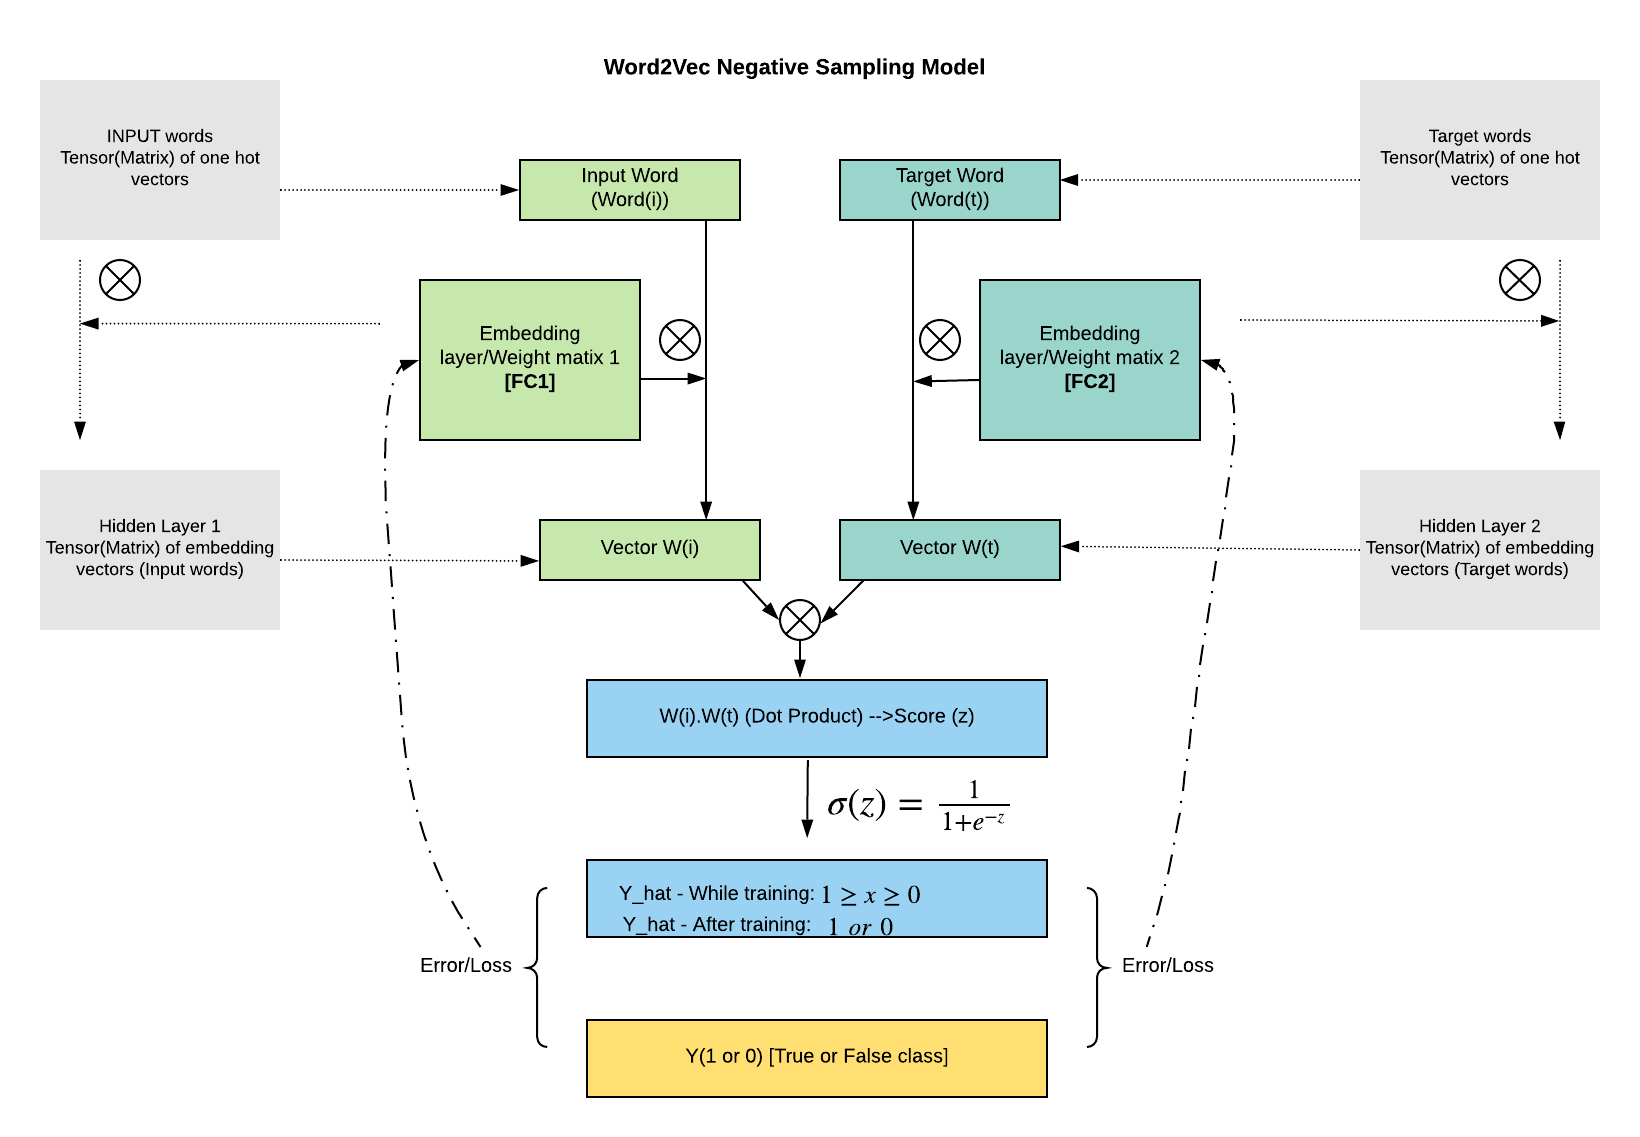
\includegraphics[width=15cm]{thesis/figures/word2vec-skip-gram-negative-sampling.png}
    \caption{TODO: Replace with TikZ illustration}
    \label{fig:word2vec-skip-gram-negative-sampling}
\end{figure}

\subsubsection{Input layers}
We have two input layers in our ANN; one for the target word $w_t$ and one for the context word $w_{t+j}$, $-R \leq j \leq R, j \neq 0$. The values to the input layers are typically one-hot encoded or represented using an integer corresponding to the index of the word in the vocabulary. For explanation purposes, we will use the one-hot encoded representation here, but in our code implementation, we use the latter one. We denote the one-hot encoded input values to the input layers to be $e_{w_t}$ and $e_{w_{t+j}}$ for the target and context input layers respectively.

\subsubsection{Hidden layer}
We have one hidden layer in our ANN. To calculate the result from the input layers to the hidden layer, we introduce two $|V| \times D$ weight matrices $W$ and $W'$, where $|V|$ is the vocabulary size and $D$ is the hidden embedding dimension. The $W$ matrix consists of weights related to the target word $w_t$ and can be though of as the "input to hidden" matrix. The $W'$ matrix consists of weights related to the context word, and unlike the $W$ matrix, it can be though of as the "hidden to output" matrix from the original introduction to negative sampling \cite{mikolov2013b}. Note that both $W$ and $W'$ are randomly initialized. Furthermore, we refer to $W$ and $W'$ as the target and context embedding matrix, respectively.

To map from the input to the hidden layer, we simply multiply the transposed of an embedding matrix with its respective one-hot encoded input vector, resulting in a "look-up" of the embedding vector. To illustrate with an example, imagine if we had the one-hot encoded vector $e_{w_t} = \left( \begin{smallmatrix}
    1\\
    0\\
\end{smallmatrix} \right)$ and the embedding matrix $W = \left( \begin{smallmatrix}
    1 & 2 & 3\\
    4 & 5 & 6\\
\end{smallmatrix} \right)$. If the multiply the transpose of the embedding matrix with the one-hot encoded vector, i.e. $\trans{W} e_{w_t}$, we would get $\left( \begin{smallmatrix}
    1\\
    2\\
    3\\
\end{smallmatrix} \right)$, essentially performing a transposed "copy" operation.

We let $v_{w_t} = \trans{W} e_{w_t}$ be the mapping for word $w_t$ and $v'_{w_t+j} = \trans{W'} e_{w_t{+j}}$ be the mapping for word $w_{t+j}$ from the inputs to the hidden layer. We refer the vectors $v_{w_t}$ and $v'_{w_{t+j}}$ to as the target and context embedding vectors, respectively. Note that when computing the embedding vectors, we do not apply any activation function (i.e. performing a linear transformation) nor any bias, leading to more efficient training of bigger datasets \cite{mikolov2013a}.

\subsubsection{Output layer}
Recall that when we are using negative sampling, we would like to ensure that words in the same context yield similar word vectors, and that words words that are not in the same context (i.e. a target word versus a word sampled from the noise distribution $P_n(w)$) to be dissimilar \cite{mikolov2013b}. From the objective of negative sampling from \cref{eqn:negative-sampling-obj-func}, we see that we use the sigmoid function on the dot product between the "input" and the "output" vectors $v$ and $v'$. When we take the dot product, we are essentially computing an unnormalized cosine similarity measure between the vectors. The idea is then to use this similarity measure and convert it into the range of $[0, 1]$ by using the sigmoid function. Following, we want similar vectors to have 1 as output from the sigmoid function and dissimilar vectors to have 0 as the output from the sigmoid function. When we compute the loss of the ANN, we generate $k$ samples from the noise distribution $P_n(w)$ such that we can use them for computing the loss of the network.

For each positive target-context pair we have in our data, we create a single sigmoid output plus $k$ sigmoid outputs for each negatively sampled word from the noise distribution $P_n(w)$. Thus, we could argue that we have $(k + 1)$ outputs in our network. As one should note, however, we are only interested in the learned embedding matrix $W$ and its corresponding word vectors; we will not use the ANN for predicting whether a certain word is more or less likely to be within a words contextual neighborhood, thus, discarding the output of the network.

Similar to \cite{mikolov2013a}, we update the embedding weights $W$ and $W'$ using the stochastic gradient descent (SGD) optimizer, adjusting all the weights of the embedding matrices during the training of the ANN to minimize the loss in \cref{eqn:skip-gram-negative-sampling-objective}. Furthermore, we use a linearly decreasing learning rate, meaning that we start out with some initial learning rate $lr$ and decrease linearly to $lr_{min}$ until we reach end of training. The linearly decreasing learing rate was also implemented by \cite{mikolov2013a}.

\subsection{Hyperparameters in word2vec}
When training a word2vec model, we have to choose several hyperparameters. In this subsection, we will go over all choices of hyperparameters and explain them.

\begin{itemize}
    \item \textbf{min-word-count} \\
        The minimum word count denotes a threshold of how many times a word at least has to occur in a text for it to be in the vocabulary. In the empirical experiments of Mikolov et al, they used 5 as the threshold \cite{mikolov2013b}.
    \item \textbf{max-vocab-size} \\
        The maximum vocabulary size denotes the maximal number of words to have in our vocabulary, sorted from most to least occurring word. We may set the maximum vocabulary size to reduce the computational complexity and to remove some less occurring words.
    \item \textbf{batch-size} \\
        Batch size is the number of positive target-context pairs $(w_t, w_{t+j})$ we train on in each training step, i.e., the number of forward passes we perform in our ANN before we do a backwards pass.
    \item \textbf{num-epochs} \\
        Number of epochs denotes the number of times we train on the training data. With word2vec, one usually sets this number rather low (e.g. $1-5$), since it has been reported that by training on more data, we need less epochs to get comparable or better quality word vectors \cite{mikolov2013a}.
    \item \textbf{learning-rate} \\
        The learning rate denotes how fast we want our weights to change in our ANN. The original authors of word2vec used 0.025 (i.e. $2.5\%$) as the initial learning rate for their experiments.
    \item \textbf{min-learning-rate} \\
        The minimal learning rate denotes how small the learning rate should be when approaching the end of the training. Mikolov et al. stated that they decreased it linearly, such that it approaches zero at the end of the last training epoch. It should be noted, however, that in the original code of word2vec, they linearly decrease the learning rate to the initial learning rate $lr$ times $0.0001$ (i.e. $0.025 \times 0.0001 = 0.0000025$)\footnote{\href{https://github.com/tmikolov/word2vec/blob/e092540633572b883e25b367938b0cca2cf3c0e7/word2vec.c\#L398}{word2vec.c at line 398 (of the original word2vec repository)}}.
    \item \textbf{embedding-dim} \\
        The embedding dimension denotes the dimension we want to use for the internal matrices $W$ and $W'$ in our ANN, i.e., the dimensionality of the word vectors.
    \item \textbf{max-window-size} \\
        Maximum window size denotes the maximal number of words to look for to the left and to the right of a target word $w_t$. Mikolov et al. reported that they used $5$ as the window size \cite{mikolov2013b}.
    \item \textbf{num-negative-samples} \\
        Number of negative samples denote how many negative samples should be generated for each positive target-context pair we train on.
    \item \textbf{sampling-factor} \\
        The sampling factor is used as a threshold to randomly discard frequently occurring words in the text corpora. A common value for this is $10^{-5}$ \cite{mikolov2013b}.
    \item \textbf{unigram-exponent} \\
        The unigram exponent is which power we raise the noise distribution $P_n(w)$ to (where the noise distribution equals the unigram distribution, in our case). Although there were no theoretical justification for this, Mikolov et al. reported that the value $\frac{3}{4}$ worked the best \cite{mikolov2013b}.
\end{itemize}

\section{Evaluating a word2vec model}
\label{sec:eval-word2vec-model}
In typical machine learning projects, it is common to set aside some of the train data to be evaluated when we have finalized the model, e.g., the test data set. In the word2vec model, however, it is not common to evaluate the models performance on some independent subset of the train data. Instead, test data sets which checks for word relatedness are more common (i.e., man is to woman as king is to queen).

In the first paper introducing word2vec, they used two test data sets; the Semantic-Syntactic Word Relationship test set (SSWR) and the Microsoft Research Syntactic Analogies Dataset (MSR). SSWR was first introduced in \cite{mikolov2013a}, consists of 8869 semantic and 10675 syntactic questions and is widely used as a test dataset. The MSR dataset was first introduced in \cite{mikolov-etal-2013-linguistic} and consists of 8000 analogy questions. For the sake of simplicity, we will only use the SSWR and the MSR test data sets when evaluating the word2vec model on word analogy questions. It should be noted, however, that there are other common test data sets as well, such as the Bigger analogy test set (BATS) from \cite{gladkova-etal-2016-analogy}.

\section{Training and evaluating our word2vec implementation}
\label{sec:training-and-eval-our-word2vec-impl}
We train and evaluate our word2vec implementation to further deepen our understanding in how to implement it in practice and how it might perform versus other implementations of word2vec. As with training any machine learning model, one usually needs to prepare some data. In our case it is not any different, and before training our word2vec model, we will in this section first go over the data preprocessing choices we have made. Furthermore, we discuss the details of our own implementation of word2vec using the Skip-gram model and negative sampling. At last we cover the specific choices of hyperparameters and compare our empirical results to results from other models.

\subsection{Data preprocessing}
\label{sec:data-preprocessing}
To train a word2vec model, one needs to have a sufficiently large dataset (and thus embedding dimensionality) to yield good quality word embeddings \cite{mikolov2013b}. In the empirical experiments of \cite{mikolov2013b}, they used an internal data set from Google News. Since this dataset is not publicly available, we instead used dumps from \cite{WikimediaDumps} and performed a number of preprocessing steps, before training on it. The dumps from Wikipedia were first downloaded and parsed using the WikiExtractor tool \cite{Wikiextractor2015}. Furthermore, we created a script using Python \cite{python3-2009} to merge and process output files from the WikiExtractor tool into a certain number of text files (in our case, equal to the number of cores, to benefit from parallel reading), such that we can train on it with ease.

We then proceed by processing each Wikipedia article. In particular, we performed the following steps
\begin{enumerate}
    \item We split each article into a list of sentences using the \textit{tokenize.sent\_tokenize} function from the NLTK library \cite{bird2009natural}.
    \item Then, we preprocess each sentence individually.
    \begin{enumerate}
        \item We first replace contractions in each sentence (e.g. I'll $\mapsto$ I will, you'd $\mapsto$ you would, etc.) by using the contractions pip-package \cite{contractions-2016}.
        \item Then we split the sentence into a list of words using the \textit{word\_tokenize} function from NLTK.
        \begin{enumerate}
            \item We convert each word in the sentence to its lower-case representation.
            \item We remove punctuation from words and create new sub-words for each word delimited by punctuation (e.g. out-of-the-box $\mapsto$ out, of, the, box).
            \item At last, we replace all numbers (including ordinal numbers) with its textual representation. For example, the number 10 becomes "ten" and the word "21st" becomes "twenty-first".
        \end{enumerate}
    \end{enumerate}
    \item With the new processed sentences, we filter out sentences that have less than \textbf{min\_word\_count} words in them.
    \item Each sentence is then appended to an output text file, separated using the newline character (i.e. \textbackslash n).
\end{enumerate}

\textbf{TODO}: Write about word2phrase.

\subsection{Implementation specifics}
To implement the word2vec model, we used Python and Tensorflow \cite{python3-2009, tensorflow2015-whitepaper}. In particular, we implemented the Skip-gram model using negative sampling. To do so, we split our implementation into three main Python classes. The first class is the \path{Tokenizer}. It is responsible for converting text into word indices in vocabulary (e.g. the word "hello" $\mapsto$ 42). The second class is the \path{Word2vecSGNSModel}, which inherits the \path{tf.keras.Model} class from Tensorflow\footnote{We created the model using subclassing, as specified in \href{https://www.tensorflow.org/guide/keras/custom_layers_and_models}{this guide from Tensorflow}.}, and is the model we use to train our ANN. The third and final main class is \path{Word2vec}. It performs training using the \path{Word2vecSGNSModel} and uses \path{Tokenizer} internally to convert words into integers.

To load the data into the model, we use the \path{tf.data} API, as introduced in Tensorflow 2. The \path{tf.data} API allows us to create flexible and scalable data generators. As mentioned in \cref{sec:data-preprocessing}, we want to train our model on dumps from Wikipedia, i.e., several gigabytes of raw text data, and the \path{tf.data} API allows us to exactly this in a quick and efficient manner. In particular, we used the \path{tf.data.TextLineDataset} class to load multiple text files in parallel and set \path{num_parallel_calls} to \path{tf.data.experimental.AUTOTUNE} wherever we could, such that we parallelize the data generation process as much as possible. We also used \path{prefetch} to prepare the data on the CPU while training.

By implementing word2vec ourselves, we learned a few things we did not realize after reading the two original papers from Mikolov et al. \cite{mikolov2013a, mikolov2013b}
\begin{itemize}
    \item Training on big datasets (e.g. dumps from Wikipedia) requires an efficient implementation of the data generator. We first attempted to create a data generator which loaded everything into memory, but it became clear to us that this does not scale well when we later want to test on bigger data sets.
    \item Preprocessing of data may drastically change the quality of the word embeddings.
    \item There are two embedding matrices $W$ and $W'$ corresponding to the input and output of the network. At first, we only had a single embedding matrix, for both the input and the output of the network.
\end{itemize}

\subsection{Hyperparameter choices}
\label{sec:hyperparameter-choices}
To train the word2vec model, we base our choices of hyperparameters to the different choices used in models from \cite{mikolov2013a, mikolov2013b}. These hyperparameters can be found in \cref{table:word2vec-hyperparameter-choices}.

\begin{table}[ht]
    \centering
    \begin{tabular}{@{}ll@{}}
    \toprule
    Hyperparameter & Value\\
    \midrule
    \rowcolor[HTML]{F5F5F5} \textbf{min-word-count} & 5\\
    \textbf{max-vocab-size} & $\infty$ \\
    \rowcolor[HTML]{F5F5F5} \textbf{batch-size} & 256\\
    \textbf{num-epochs} & 5\\
    \rowcolor[HTML]{F5F5F5} \textbf{learning-rate} & 0.025\\
    \textbf{min-learning-rate} & 0.0000025\\
    \rowcolor[HTML]{F5F5F5} \textbf{embedding-dim} & 300\\
    \textbf{max-window-size} & 5\\
    \rowcolor[HTML]{F5F5F5} \textbf{num-negative-samples} & 5\\
    \textbf{sampling-factor} & 0.00001\\
    \rowcolor[HTML]{F5F5F5} \textbf{unigram-exponent} & 0.75\\
    \bottomrule
    \end{tabular}
    \caption{Hyperparameters used to train our word2vec model}
    \label{table:word2vec-hyperparameter-choices}
\end{table}

Similar to \cite{mikolov2013b}, we set the minimum word count to 5, i.e., we discard words that occur less than 5 times in the data we train on. In addition to this, we did not restrict the maximum vocabulary size, e.g., we let the vocabulary include any words that occur at least 5 times.

Neither \cite{mikolov2013a} nor \cite{mikolov2013b} stated which batch-size they used, but by inspecting the original source code\footnote{\href{https://github.com/tmikolov/word2vec/blob/e092540633572b883e25b367938b0cca2cf3c0e7/word2vec.c/\#L542}{word2vec.c at line 542 (of the original word2vec repository)}}, we concluded that they used 1 as their batch size, e.g., performing a backward pass for every forward pass in the model. We found, however, that setting the batch size to 256 to be a nice fit for our data, leading to good quality vectors and faster training.

Mikolov et al. used 1 to 4 epochs in their experiments \cite{mikolov2013a, mikolov2013b}, and in the original source code of word2vec\footnote{\href{https://github.com/tmikolov/word2vec/blob/e092540633572b883e25b367938b0cca2cf3c0e7/word2vec.c/\#L43}{word2vec.c at line 43 (of the original word2vec repository)}}, they default to 5 epochs. For this reason, we set the number of epochs to 5.

We set the initial and minimum learning rate to 0.025 and 0.000025, respectively, as noted in \cite{mikolov2013a} and the original source code of word2vec.

Furthermore, we set the embedding dimension to 300, the maximal window size to 5, the number of negative samples to 5, the sampling factor to 0.00001 and the unigram exponent to 0.75, similar to experiments from \cite{mikolov2013b}.

Using the preprocessing steps from \cref{sec:data-preprocessing} on our data and the hyperparameters from \cref{table:word2vec-hyperparameter-choices}, we get a vocabulary size of 1682564 ($\sim$1.7M) and corpus size of 2514127336 ($\sim$2.5B).

\subsection{Empirical results}
We evaluated a word2vec model trained on the hyperparameters from \cref{sec:hyperparameter-choices} on a machine with a single GPU (GeForce RTX 2080 Ti), one CPU (Intel i9-7900X @ 3.30GHz) and 64 GB of RAM. We evaluated the trained model using the SSWR and MSR test datasets and compare the results to models from \cite{mikolov2013a, mikolov2013b, mikolov-etal-2013-linguistic, bojanowski2017enriching}. In particular, we compare to the Skip-gram models from \cite[Table 3]{mikolov2013a} and \cite[Table 6]{mikolov2013a} (denoted SG 300 and 1000 respectively), the NEG-15 model from \cite[Table 1]{mikolov2013b}, the RNN-1600 model from \cite[Table 2]{mikolov-etal-2013-linguistic} and the fastText model from \cite[Table 2]{bojanowski2017enriching}. \textbf{TODO}: Write something about fastText? The results are shown in \cref{table:word2vec-eval-empirical-results} (a dash denotes that the model has not been evaluated on the particular subset/data set).

\begin{table}[ht]
    \centering
    \begin{tabular}{@{}cm{1.7cm}m{1.7cm}m{1.7cm}m{1.7cm}m{1.7cm}m{1.7cm}m{1.7cm}@{}}
    \toprule
    & \multicolumn{3}{c}{\cite[SSWR]{mikolov2013a}} & \multicolumn{4}{c}{ \cite[MSR]{mikolov-etal-2013-linguistic}} \\ \cmidrule(l){2-8} 
    \multirow{-2}{*}{Model} & Semantic Accuracy {[}\%{]} & Syntactic Accuracy {[}\%{]} & Total Accuracy {[}\%{]} & Adjectives Accuracy {[}\%{]} & Nouns Accuracy {[}\%{]} & Verbs Accuracy {[}\%{]} & Total Accuracy {[}\%{]} \\ \midrule
    \rowcolor[HTML]{F5F5F5}
    SG 300 & 55 & 59 & -- & -- & -- & -- & \textbf{56} \\
    SG 1000 & 66.1 & 65.1 & 65.6 & -- & -- & -- & -- \\
    \rowcolor[HTML]{F5F5F5}
    NEG-15 & 61 & 61 & 61 & -- & -- & -- & -- \\
    RNN-1600 & -- & -- & -- & 23.9 & 29.2 & \textbf{62.2} & 39.6 \\
    \rowcolor[HTML]{F5F5F5}
    fastText & \textbf{77.8} & \textbf{74.9} & -- & -- & -- & -- & -- \\
    Our model & 70.1 & 64.3 & \textbf{66.4} & \textbf{42.2} & \textbf{67.6} & 58.2 & \textbf{56} \\
    \bottomrule
    \end{tabular}
    \caption{Comparison of empirical results on the SSWR and MSR word analogies test data sets.}
    \label{table:word2vec-eval-empirical-results}
\end{table}

\textbf{TODO}: Comment on the result.